%============================================================================
% tento soubor pouzijte jako zaklad
% (c) 2008 Michal Bidlo
% E-mail: bidlom AT fit vutbr cz
%============================================================================
% kodovaní: iso-8859-2 (zmena prikazem iconv, recode nebo cstocs)
%----------------------------------------------------------------------------
% zpracování: make, make pdf, make desky, make clean
% p?ipomínky posílejte na e-mail: bidlom AT fit.vutbr.cz
% vim: set syntax=tex:
%============================================================================
\documentclass[english]{fitthesis} % odevzdani do wisu - odkazy, na ktere se da klikat
%\documentclass[cover,print]{fitthesis} % pro tisk - na odkazy se neda klikat
%\documentclass[english,print]{fitthesis} % pro tisk - na odkazy se neda klikat
%      \documentclass[english]{fitthesis}
% * Je-li prace psana v anglickem jazyce, je zapotrebi u tridy pouzit 
%   parametr english nasledovne:
%\documentclass[cover][english]{fitthesis}
% * Neprejete-li si vysazet na prvni strane dokumentu desky, zruste 
%   parametr cover

% zde zvolime kodovani, ve kterem je napsan text prace
% "latin2" pro iso8859-2 nebo "cp1250" pro windows-1250, "utf8" pro "utf-8"
%\usepackage{ucs}
\usepackage[utf8]{inputenc}
\usepackage[T1, IL2]{fontenc}
\usepackage{url}
\DeclareUrlCommand\url{\def\UrlLeft{<}\def\UrlRight{>} \urlstyle{tt}}

%zde muzeme vlozit vlastni balicky
\usepackage{lineno}
\usepackage{color}
%definice lstlisting
\usepackage{listings}

\def\lstlistingname{Example}
\definecolor{gray}{rgb}{0.4,0.4,0.4}
\definecolor{darkblue}{rgb}{0.0,0.0,0.6}
\definecolor{cyan}{rgb}{0.0,0.6,0.6}
\lstdefinelanguage{XML}
{
 morestring=[b]",
 morestring=[d]{>}{<},
 morecomment=[s]{<?}{?>},
 stringstyle=\color{black},
 identifierstyle=\color{darkblue},
 keywordstyle=\color{cyan},
 morekeywords={xmlns,version,type, message, from, to, body, iq, stream, mechanism, presence, status,xml:lang, item, jid, query,show}% list your attributes here
}
\lstset{
  basicstyle=\ttfamily,
  columns=fullflexible,
  showstringspaces=false,
  commentstyle=\color{gray}\upshape
}
\lstset{ %
language=XML, % the language of the code
%basicstyle=\footnotesize, % the size of the fonts that are used for the code
numbers=left, % where to put the line-numbers
numberstyle=\footnotesize, % the size of the fonts that are used for the line-numbers
stepnumber=1, % the step between two line-numbers. If it's 1, each line will be numbered
numbersep=10pt, % how far the line-numbers are from the code
backgroundcolor=\color{white}, % choose the background color. You must add \usepackage{color}
showspaces=false, % show spaces adding particular underscores
showstringspaces=false, % underline spaces within strings
showtabs=false, % show tabs within strings adding particular underscores
frame=tb, % adds a frame around the code
tabsize=2, % sets default tabsize to 2 spaces
captionpos=b, % sets the caption-position to bottom
breaklines=true, % sets automatic line breaking
breakatwhitespace=false, % sets if automatic breaks should only happen at whitespace
title=\lstname, % show the filename of files included with \lstinputlisting; also try caption instead of title
escapeinside={\%*}{*)}, % if you want to add a comment within your code
morekeywords={*,...}, % if you want to add more keywords to the set
commentstyle=\color{gray}\upshape
}

% =======================================================================
% balí?ek "hyperref" vytvá?í klikací odkazy v pdf, pokud tedy pou?ijeme pdflatex
% problém je, ?e balí?ek hyperref musí být uveden jako poslední, tak?e nem??e
% být v ?ablon?
\ifWis
\ifx\pdfoutput\undefined % nejedeme pod pdflatexem
\else
  \usepackage{color}
  \usepackage[unicode,colorlinks,hyperindex,plainpages=false,pdftex]{hyperref}
  \definecolor{links}{rgb}{0.4,0.5,0}
  \definecolor{anchors}{rgb}{1,0,0}
  \def\AnchorColor{anchors}
  \def\LinkColor{links}
  \def\pdfBorderAttrs{/Border [0 0 0] }  % bez okraj? kolem odkaz?
  \pdfcompresslevel=9
\fi
\fi

%Informace o praci/projektu
%---------------------------------------------------------------------------
\projectinfo{
  %Prace
  project=SP,            %typ prace BP/SP/DP/DR
  year=2011,             %rok
  date=\today,           %datum odevzdani
  %Nazev prace
  title.cs={VoIP v jabber klientu},  %nazev prace v cestine
  title.en={VoIP in jabber client}, %nazev prace v anglictine
  %Autor
  author={Vojtěch Kulička},   %jmeno prijmeni autora
  author.title.p=Bc., %titul pred jmenem (nepovinne)
  %author.title.a=PhD, %titul za jmenem (nepovinne)
  %Ustav
  department=UPGM, % doplnte prislusnou zkratku: UPSY/UIFS/UITS/UPGM
  %Skolitel
  supervisor={Jozef Mlích}, %jmeno prijmeni skolitele
  supervisor.title.p={Ing.},   %titul pred jmenem (nepovinne)
  %supervisor.title.a={},    %titul za jmenem (nepovinne)
  %Klicova slova, abstrakty, prohlaseni a podekovani je mozne definovat 
  %bud pomoci nasledujicich parametru nebo pomoci vyhrazenych maker (viz dale)
  %===========================================================================
  %Klicova slova
  keywords.cs={VoIP, IM, sdílená tabule, XMPP, telepathy}, %klicova slova v ceskem jazyce
  keywords.en={VoIP, IM, Shared whiteboard, XMPP, telepathy}, %klicova slova v anglickem jazyce
  %Abstract
  abstract.cs={Práce se zabývá možnostmi přidání funkcionality do existujícího XMPP programu se sdílenou tabulí. Analyzuje možnosti využití současných technologií pro podporu VoIP. Cílem je port klienta na komunikační architekturu telepathy a implementace VoIP.}, % abstrakt v ceskem jazyce
  abstract.en={This thesis tackles the issues of implementing a VoIP support into an XMPP based IM application. The state of the art is analyzed to find a suitable technology to base the VoIP on. The work's goal is to port the existing client application to network framework telepathy and implentation of VoIP.}, % abstrakt v anglickem jazyce
  %Prohlaseni
  declaration={Prohlašuji, že jsem tuto diplomovou práci vypracoval samostatně pod vedením pana inženýra Jozefa Mlícha},
  %Podekovani (nepovinne)
  acknowledgment={Děkuji svému vedoucímu Ing.Jozefu Mlíchovi a Ing.Jaroslavu Řezníkovi za odbornou pomoc. } % nepovinne
}

%Abstrakt (cesky, anglicky)
%\abstract[cs]{Do tohoto odstavce bude zapsán výtah (abstrakt) práce v ?eském jazyce.}
%\abstract[en]{Do tohoto odstavce bude zapsán výtah (abstrakt) práce v anglickém jazyce.}

%Klicova slova (cesky, anglicky)
%\keywords[cs]{Sem budou zapsána jednotlivá klí?ová slova v ?eském jazyce, odd?lená ?árkami.}
%\keywords[en]{Sem budou zapsána jednotlivá klí?ová slova v anglickém jazyce, odd?lená ?árkami.}

%Prohlaseni
%\declaration{Prohla?uji, ?e jsem tuto bakalá?skou práci vypracoval samostatn? pod vedením pana X...
%Dal?í informace mi poskytli...
%Uvedl jsem v?echny literární prameny a publikace, ze kterých jsem ?erpal.}

%Podekovani (nepovinne)
%\acknowledgment{V této sekci je možno uvést poděkování vedoucímu práce a těm, kteří poskytli odbornou pomoc
%(externí zadavatel, konzultant, apod.).}

\begin{document}
  % Vysazeni titulnich stran
  % ----------------------------------------------
  \maketitle
  % Obsah
  % ----------------------------------------------
  \tableofcontents
  
  % Seznam obrazku a tabulek (pokud prace obsahuje velke mnozstvi obrazku, tak se to hodi)
  % \listoffigures
  % \listoftables 

  % Text prace
  % ----------------------------------------------
  %==========================================================================================================================
% (c) Vojtěch Kulička, 2010

\chapter{Introduction}
Human is a social creature and likes to chat, share feelings and ideas. At first we managed to do so by making simple sounds. Those sounds later on developed into words. Then much later the human race started to feel the need to record what we were thinking. We made up symbols and started to write. As the society grew and spread, we wanted to communicate with people from other tribes and villages. At first we would travel and use spoken words, but as the distances grew we figured we can have our thoughts delivered in writing. Mail was born. In 1844 telegraph was invented by Samuel Morse followed by telepthone in 1874 by Alexander Graham Bell. And finally in 1969 the Internet was created. All of these inventions aimed to provide means of communication to satisfy the needs of the evolving society.  

In the early days of the Internet email was the main means of communication. And just like regular mail people would have their electronic mailboxes to which the emails were delivered. Email was a huge step forward for it provided a way to almost instantly deliver text from one place to another regardless of the distance for free. The main disadvantage of email is that people had to check their mailboxes read new mail and then reply. It is just neither fast nor convenient enough for team cooperation when team members are far apart. For those and other purposes like chatting Instant Messenger programs were introduced.    

An IM program offers realtime communication between two people via text messages that are delivered from one user to another instantly. Instant messangers became very popular and started adding on features like multiuser chat, various games and most importantly VoIP(Voice over IP) support. VoIP capable IM like skype have become extremely popular at first for making it possible for people to call each other for free over the internet. Later video conferencing capability was added, so you could talk and see you colleague at the same time. One more thing comes in extremely handy when working in a team - a whiteboard.

At this time there is no usable IM providing VoIP and shared whiteboard for GNU/Linux. This thesis aims to add VoIP support to an existing XMPP client with shared board called Makneto. Makneto was created by Jaroslav Řezník as a master's thesis in 2008. At this point it is using iris library for XMPP communication. The shared board data is also transferred over XMPP. One of the goals of this thesis is to port Makneto to telepathy, which is now a very reliable and robust library for communication for numerous protocols.  

The following chapter gives a detailed description of the current version of program Makneto. We will find out about it's architecture, strengths and weaknesses. 

Chapter number three focuses on XMPP/Jabber communication protocol. It talks about it's features and limitations. 

Chapter three is about Telepathy communiation framework, how it works, what it consists of. There is also a description of a IM client application Empathy based on Telepathy. 

Current audio and video streaming protocols are listed and discussed in chapter five. Based on this chapter a suitable protocol is chosen for the implementation.

Finally the implementantion of VoIP into Makneto is in chapter six.  

% =========================================================================================================================
% =========================================================================================================================

\chapter{Makneto}
\section{Current architecture}
Makneto is an instant messenger with a shared board capability. It was written by Jaroslav Řezník as his master's thesis in 2008. Makneto is written in C++ using Qt version 4 and KDE 4 libraries. Qt is a application framework written in C++. Qt extends C++ and instead of callback function uses a concept of signals and slots, which is as opposed to callback functions type-safe. It runs on all major computer platforms like GNU Linux, Microsoft Windows and Mac OS X. Moreso it is supported by mobile device platforms such as Symbian and Microsoft Windows Mobile. There is also a port to Google Android called Lighthouse. Qt was developed by company named Trolltech and was available under two licenses. First was a commercial license allowing companies to write proprietory applications for a fee. Second was GNU General Public License, which was of course free. Thanks to the commercial license the Qt documentation is one of the best among any software available under GNU GPL. In june 2008 Troltech was acquired by Nokia. Nokia decided to make the source code available so that anyone could contribute. In January 2009 with the release of Qt 4.5 another licensing option was added - Lesser General Public License.\cite{wikiQt}\cite{Qt}

Besides Qt Makneto utilizes functionality provide by KDE 4\cite{KDE} libraries, which makes Makneto unable to run on a different operating system than GNU Linux. KDE is a desktop environment created by Matthias Ettricht in 1996 for he felt the need for a good quality window manager for Linux. KDE is currently in version 4, which brought great features. There is a new desktop called Plasma, which allows users to display widgets called plasmoids directly on the desktop. That allows users to have a TODO list, calendar, translator, weather forecast, system monitor and much more right in front of them on their desktops without having launch any of those to get the information they need. It makes users' work eesier and more efficient. KDE and GNOME are the most common window manager in Linux. GNOME offers stable useful environment and is influenced mostly by large businesses using it. KDE is more flexible and works more with the look and feel.

Makneto communicates using XMPP/Jabber protocol implemented in Qt-based C++ library called Iris. All of the Iris is primarily used by Psi instant messenger. It's development is still quite active and it supports all of Jabber's key features. Iris' downside is very poor documentation. It's wiki is very brief and all to all gives one example. The only way to find out how it works is browsing through Psi code.\cite{irisWiki}

Makneto's shared whiteboard is based an official extension of XMPP SVGWB by Joonas Govenius\cite{SVGWB}. SVGWB is implemented in Psi and Makneto utilizes their code. SVGWB defines all the necessary actions like whiteboard session initianion including invitation and mainly how to send and receive information about the grahical objects using XMPP text messages. The actual graphical object representation is defined by SVG\cite{SVG}(Scalable Vector Graphics) by W3C. SVG describes graphics objects using vectors in XML format. Makneto uses just a subset of SVG called SVG Tiny\cite{SVGtiny} as it does not need all of the features of SVG. Tiny SVG describes two-dimensional vector graphics and raster graphics and multimedia. To sum up Makneto's whiteboard features, it allows you to draw lines, rectangles, elipses, circles, sketch using a paintbrush and input images in jpg and png formats. Graphical objects are resizeable, can be rotaded and copied.  


Makneto runs in one window. User's contact list is on a panel on the left hand side. The whiteboard and chat session are initiated through the contact list. Makneto handles more session at once each in a separate tab. Using the application is very comfortable although it from dies time to time.

% (see figure \ref{fig:makneto})
%TODO - pic of makneto


\section{Motivation for porting and adding VoIP support}
Makneto has a potential to become a great collaboration tool. The tasks of today are more and more dificult so the need to solve the task in teams is greater and greater. Especially in comupter science the teams are ofter from all over the world and it is important to discuss current issues. Meeting in person is not an option and that is where Makneto comes in. The shared whiteboard is very useful for sharing thinkmaps and visualising problems and solutions, but the days when people had the time and patience to write are gone. Everybody wants to talk these days.  

Makneto is at this point has couple design flaws. First it uses iris library for communication in XMPP network. Iris is very poorly documented and every change in the implementation would reflect in Makneto. Second Makneto depends on KDE libraries, which at this point is not necessary. Getting rid of this dependancy will help increase Makneto's portability. 

The current implemenation of Makneto is UI and backend in one large application. The goal is to separate the backend and UI. Backend will take care of communication. That means text messaging, shared whiteboard and after this thesis is finished also VoIP. Backend will use communications framework telepathy described in the following chapter. Telepathy supports various protocols as well as voice and video calls. Makneto will be able to use XMPP, ICQ, IRC, MSN etc. with one implementation of a client.

Frontend shall be a subject to change based on target device. Makneto for PC will have a Qt4 frontend and Makneto for smartphones and tablets will use the Qt Quick UI. With rapidly increasing number tablets and smartphones made and sold it would be shame not to plan to support them.  




% =========================================================================================================================
% =========================================================================================================================

\chapter{XMPP}
This chapter talks about Extensible Messaging and Presence Protocol\cite{xmpp}, it's history, key features and usage. The information is mailny acquired from from \cite{xmppBook,xmppCoreRFC,xmppIMRFC}.

\section{History}
In 1999 Jerremie Miller created protocol called Jabber. Jabber was an open protocol based on XML as opposed to existing protocols like ICQ\cite{ICQ} or AIM\cite{AIM}, which were proprietory and owned and controlled by private companies. The first attemp to make Jabber a standard failed. The second attempt did not use the name Jabber, but eXtensible Messaging and Presence Protocol instead. IETF\footnote{Internet Engineering Task Force} approved and XMPP was standardized in 2004 in RFC 3920 and RFC 3921 called XMPP Core and XMPP IM respectively. Development of XMPP is still active as it is based on XML it is possible to add functionality without jeopardising the compatibility of existing implemenstations.      

\section{XMPP protocol}
XMPP is defined in \cite{xmppCoreRFC} and \cite{xmppIMRFC}, which describe all the key features of the protocol. Authors of XMPP aim for a scalable, extensible and in every way powerful protocol. Years later with XMPP still around and more and more popular we can safely say they succeeded. The key features of XMPP include:

\begin{itemize}
	\item \textbf{Decentralized architecture} - XMPP network does not rely on one server. The network consists of servers and clients. Every client may run his or her own server. XMPP server registers clients and communicates with other servers much like with email(see figure \ref{fig:xmpp-decentralized-architecture}). A client often wants to communicate with another client on a different server. In such case other client's server is looked up and the message forwarded. If a client is not satisfied with the server he or she registered with he or she may simply register with a different server or run his or her own. There is also no way to take the whole network out with DoS\footnote{Denial of Service} attack. There simply is not a small number of target to attack.    
	\item  \textbf{Open nature} - XMPP is an open standard that can be used by anyone without having to pay, sign any agreement or behave by any restrictive policies. Also it's fate is not in hands of one company but rather in the hands of everyone. Anyone who wishes to contribute can do so by cooperating with XMPP Standards Foundation. 
	\item \textbf{Extensibility} - thanks to XML based nature of XMPP it is very simple to add new features without discontinuing support of the old ones. This feature makes XMPP very flexible for it can easily add new functionality and it has been already done couple times.  
	\item \textbf{Security} - with built-in support for TLS and SSL there is no need to worry that the messages might be read by a third person using man in the middle attack. Companies using XMPP for communication inside their network might run their server localy with no access to the outside world.  
\end{itemize}

\begin{figure}[ht]
\begin{center}
	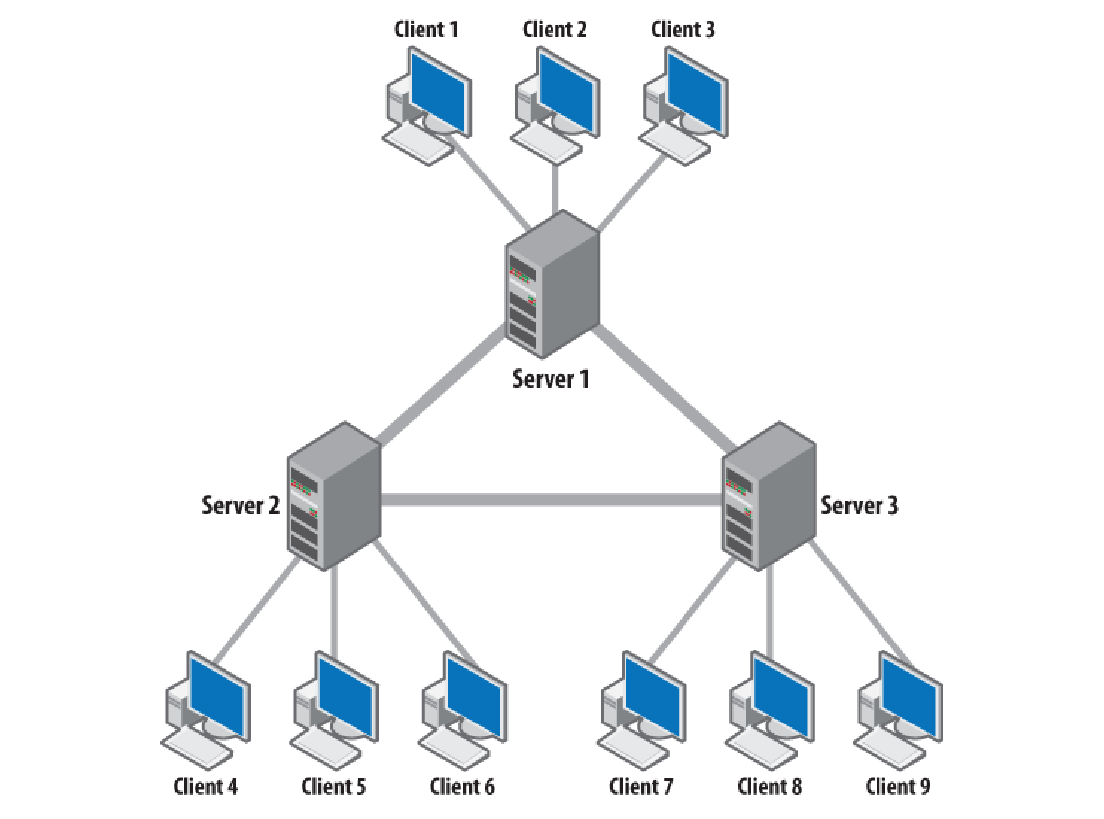
\includegraphics[width=10cm]{fig/XMPP-decentralized-architecture.png}
	\caption{XMPP decentralized architecture\cite{xmppBook}}
	\label{fig:xmpp-decentralized-architecture}
\end{center}
\end{figure}

Now let's look at the protocol and how to use it. 

\subsection*{Client-server communication}
XMPP is basicaly streaming XML documents. The stream is an unbounded XML document which contains another XML documents from both client and server. The XML documents enclosed in the stream tags with a depth of 1 are called stanzas. Stanza is a basic unit of communication like a packet. The following stanzas are defined:

\begin{itemize}
	\item \textbf{message} - used for getting information from one place to another in a push manner. The message stanza is not acknowleged and no answer is expected. It is used for instant messages, alerts, notifications, groupchat etc. The nature of the message is specified by \verb|type|.  
	\item \textbf{presence} - stanza for acquiring another user's presence. XMPP honors usess' privacy and to get someone's presence status he or she need to authorize it first by adding the querier to his or her contact list. There are several types of presence just like in any other IM protocol.     
	\item	\textbf{IQ} - is an abbreviation for Info/Query. This stanza is used for everything else. IQ works on question-answer basis. It is used for example for getting remote client's capabilities. IQ stanza must always receive a reply. 
\end{itemize}

First a TCP connection is established between client and server. Once established a stream is opened by client by sending the server \verb|<stream>| tag. There is an example of opening a stream below: 

\lstinputlisting[language=xml]{client-stream.xml}

Server answers with a second stream back to the client, which is shown in the piece of XML code that follows. 

\lstinputlisting[language=xml]{server-stream.xml}

The next step is to negotiate properties of the stream. The server sends an XML enclosed in \verb|stream:feature| tags, informing the client about features it supports. The most important property is by far encryption and authentication. Preferred encryption method is TLS, but SSL is also an option. However some servers may require usage of TLS. TLS is recommended for both client-server and server-server communication. Authentication is a key responsibility of the server. The server must ensures that users attempting to connect to it are who they say they are. The server acts as a gateway to the entire network and must not allow identity spoofing. Authentication is done via SASL\footnote{Simple Authentication and Security Layer} and options supported by the server are enclosed in \verb|mechanism| tags. The example, where server supports TLS and SASL using PLAIN text or MD5 is shown below:   

\lstinputlisting[language=xml]{starttls.xml}

Once stream parameters are set, client can request presence, set his or her own presence and communicate with other clients. Sending a message to a fellow user is accomplished via \verb|message| stanza and may look like this:

\lstinputlisting[language=xml]{sendmsg.xml}

It must include \verb|to|, \verb|from| attributes and \verb|body| opening and closing tags. The first specifis who the message is addressed to using a Jabber ID. Jabber ID consists of \verb|user name @ domain name| and many people mistake for email address. A simple Jabber ID is \verb|vtheman@jabbim.cz|. Attribute from naturaly contains a jabber ID as well, but this time an ID of the sender. The \verb|body| element contains the actual message. 
%TOTO JID
Next stanza is presence and it is needed for following presence of the contacts in the users' roster. To get presence of a user he or she must approve of it. Once user has been authorized to get another users presence they have both subscribed to get each other's presence. After connecting to the server a user sends initial presence stanza: \verb|<presence/>|. From that moment on the server takes care of the presence. Whenever the user's presence changes, it sends notification to all subscribers in the user's roster. Similarly if someone else's presence changes the user gets notified by his or her server. 

\lstinputlisting[language=xml]{presence.xml}

Presence stanza contains elements \verb|show| and \verb|status|. \verb|show| can be either \verb|chat| meaning available and ready for chat, \verb|away| meaning the user is not at the PC at the moment, \verb|xa| indicates the user will be gone for a longer period of time and finaly \verb|dnd|, which stands for do not disturb.  

The last of stanzas is Info/Query shortly IQ. IQ is very similar to HTTP in methods and in the query-answer nature. IQ queries use method \verb|get| for requesting information and method \verb|set| for making requests based on provided information. Answer to a query is IQ stanza of type \verb|result| and contains information requested by \verb|get| method or acknowledge in case of \verb|set| method. The last type of IQ is \verb|error| and is used to indicate that something went wrong. A good example of an IQ stanza is acquiring a roster: 

\lstinputlisting[language=xml]{get-roster.xml}

And the server replies with:

\lstinputlisting[language=xml]{send-roster.xml}

The stream ends with \verb|</stream>| tag and that means end for the communication. 

%\section{Jingle}

\section{Summary}
XMPP is a robust, scalable, secure, open and extensible protocol that has been well tested over the years passing all of the test without any sign of trouble. It has been very well though out and altogether it is a great protocol. The description given above is in some of the parts simplified. Full description is out of the scope of this thesis.   

% XMPP Jingle
% XMPP XEP

% =========================================================================================================================
% =========================================================================================================================

\chapter{Telepathy}
Telepathy\cite{telepathy} is a modular communications framework for building real-time communication applications. It supports numerous communication protocols as plugable backends e.g XMPP/Jabber(telepathy-gabble), SIP(telepathy-sofiasip), MSN(telepathy-butterfly) etc. Each of telepathy's components runs in a separate process as desktop service and communicates via D-Bus. The components are shared by telepathy clients. For example if there are two clients using XMPP they both use the same instance of telepathy-gabble. To get a better idea of how this concept works take a look at figure ~\ref{fig:telepathyArchitecture}.\cite{TPWiki} 

\begin{figure}[ht]
\begin{center}
	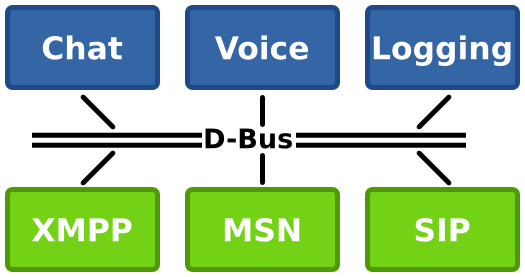
\includegraphics[width=10cm]{fig/telepathy-architecture-overview.png}
	\caption{Telepathy architecture\cite{TPWiki}}
	\label{fig:telepathyArchitecture}
\end{center}
\end{figure}


There are several features making telepathy very useful as a communications framework.

\begin{itemize}

	\item {\bf Robustness} - all the components are independent. If one crashes, others will not be affected

	\item {\bf Ease of development} - the components can be replaced without having to stop the service 

	\item {\bf Language independence} - since telepathy components use D-Bus for communication among themselves, any language that has D-Bus binding might be used to write them

	\item {\bf Desktop independence} - D-Bus is present in both main Linux window managers GNOME and KDE, so the same telepathy components could be backend for appropriate frontends.

	\item {\bf Code reuse} - the client applications do not have to worry about protocol specifics, which are handled by Telepathy. The client can use more protocols by making no or small alterations to the code.

	\item {\bf Connection reuse} - more than one Telepathy client can use the same connection simultaneously:
\end{itemize}

\section{Telepathy basic terminology}
Telepathy is a very powerful framework and as such it is also complicated. To successfuly write programs using Telepathy we need to know what telepathy consists of and what it is based on. 

\subsection*{D-Bus}
D-Bus is a kind of inter-process communication. It allows two applications running in different processes, written in different programming language communicate. More so these applications may communicate directly, without having to go through message bus daemon. There two types of D-Bus. First is a system bus used for events such as ``USB device disconnected'' or ``printer out of paper.'' Second type is per-user-login-session bus, which is used by user applications. D-Bus low level API is represented by libdbus and it requires XML parser(libxml or expat) to work. Higher level language bindings such as Qt, GLib, Java etc. are built on top of libdbus and offer more convenient way of using D-Bus, although they add more dependencies.\cite{dbus}\cite{TPWiki} 

Each process that wants to communicate over D-Bus will need to use most the following depending on it's nature: 
\begin{itemize}
	\item {\bf Unique name} - is an unique id(e.g. 2.1) assigned by D-Bus daemon to the client application. Unique name is similar to a public IP address.
	\item {\bf Wellknown name} - is similar to a DNS name. If a process wants to make a service available to other processes it requsets a wellknown name. If another process wants to access the service it uses the wellknown name to do so. Wellknown name might look like this: org.freedesktop.Telepathy.ChannelDispatcher.    
	\item {\bf Object path} - is a path to an object that is exported by process running a service.
	\item {\bf Interface} - is a way of requesting a service using signals or methods. Each D-Bus client must register at least one interface and each interface provides at least one method or signal. Every interface needs to have to name like a wellknown name.  
	\item {\bf Method} - is impleneted in the object specified by object path and exposed in the interface for that object for other processes to use. 
	\item {\bf Signal} - is a D-Bus signal client process can connect to it's callback function. If a signal is invoked the callbacked function is called.
	\item {\bf Property} - is used for exposing D-Bus object's properties. To do so the objet must implement org.freedesktop.DBus.Properties interface.
\end{itemize}

The following figure \ref{fig:dbusArchitectureNames} shows an example of two programs connected to D-Bus to be able to communicate with each other. Program B provides a service called org.freedesktop.foo.Bar(wellknown name) and it's id is 1.3. Program A does not provide any service and thus does not need any wellknown name. It just needs an id(1.2) to use other programs' services.\cite{TPWiki}

\begin{figure}[ht]
\begin{center}
	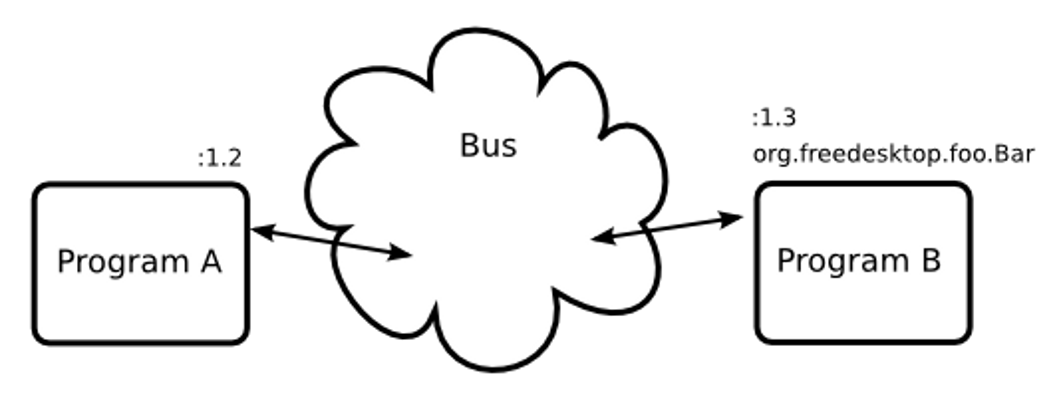
\includegraphics[width=11cm]{fig/dbus-architecture-names.png}
	\caption{D-Bus id and wellknown name example\cite{TPWiki}}
	\label{fig:dbusArchitectureNames}
\end{center}
\end{figure}


The figure \ref{fig:dbusArchitecture} shows an overview of all of the terms described above in a simple diagram.

\begin{figure}[ht]
\begin{center}
	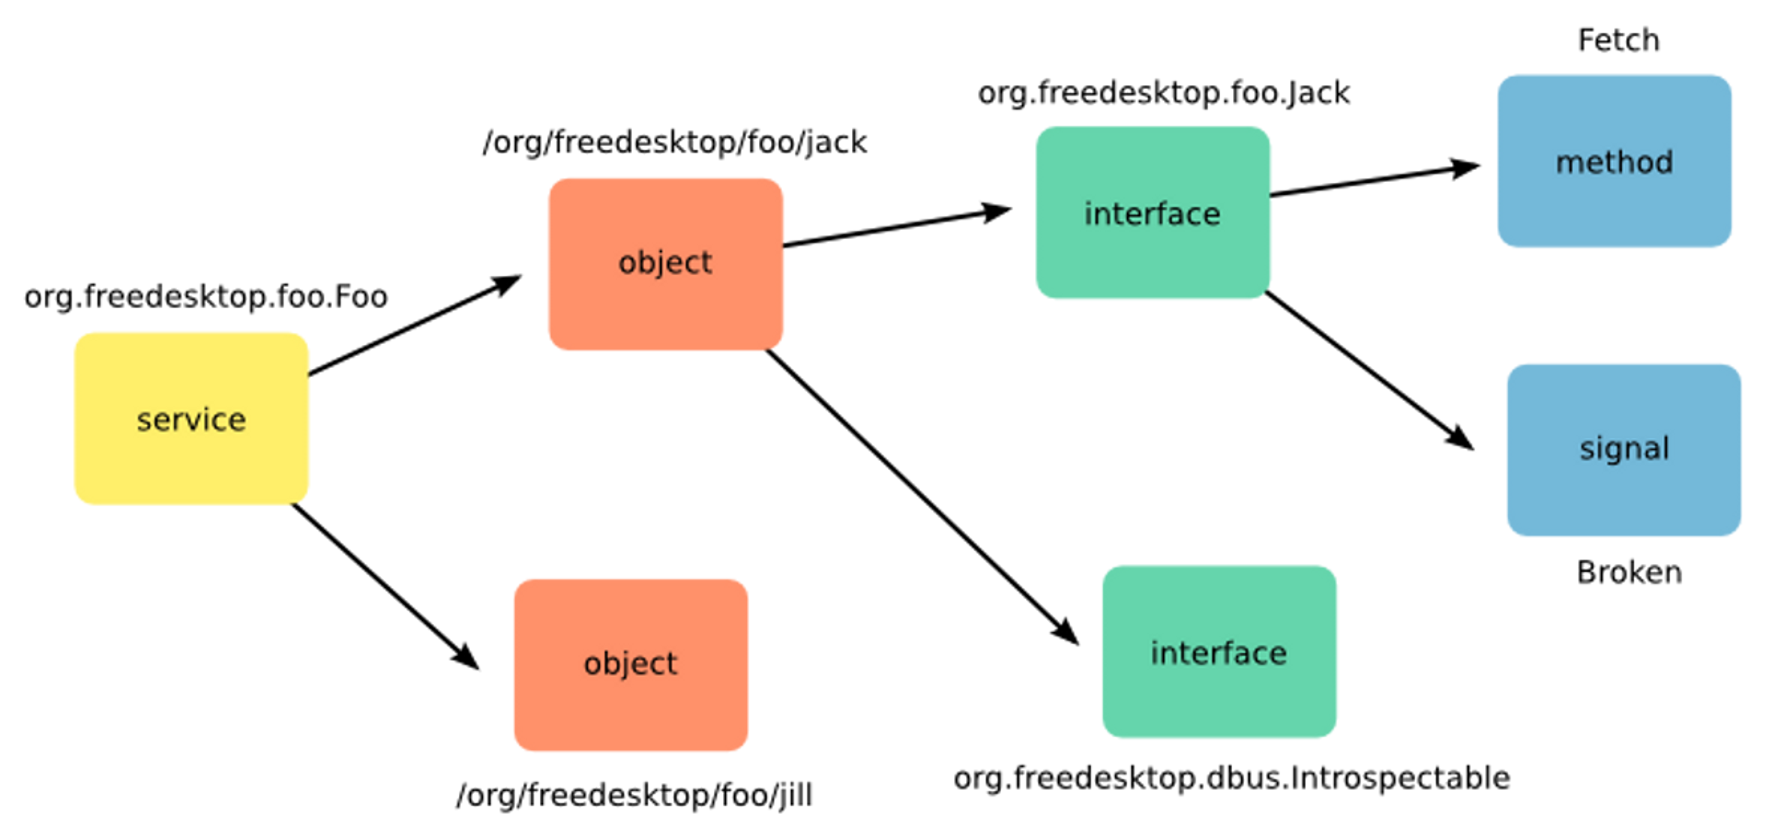
\includegraphics[width=15cm]{fig/dbus-architecture-overview.png}
	\caption{D-Bus architecture\cite{TPWiki}}
	\label{fig:dbusArchitecture}
\end{center}
\end{figure}

D-Bus is a key component of Telepathy framework. Telepathy supports many protocols all of which might provide different capabilites. For example IRC does not support avatars while XMPP does. Eventhough avatar feature is supported by XMPP protocol it might not be supported by the server we are connected to or by the opposite client in case of peer-to-peer connection. The available features are exposed by D-Bus Properties Interface. That is an easy way of determining the protocol, server or client capabilities.\cite{dbus}

\subsection*{Mission Control}
Mission Control is a Telepathy component that implements Account Manager and Channel Dispather and it's primary purpose is to encapsulate those two.\cite{TPWiki}

\subsection*{Account Manager}
Account Manager is responsible for handling accounts(e.g. XMPP, ICQ, MSN etc.). It is accessible by well-known name on D-Bus - org.freedesktop.Telepathy.AccountManager. A client application first creates an account using the CreateAccount() method, supplying it with ConnectionManager, protocol and display name. Account Manager creates and then as long as the account is active maintains Connection to that account. To create a Connection a Connection Manager is called. An account may be valid or invalid. Valid accounts may establish a Connection, whereas invalid can't. The list of valid and invalid accounts is accessible via ValidAccounts and InvalidAccounts properties respectively.\cite{TPWiki} 

\subsection*{Account}
When the Account Manager's CreateAccount() is called it returns an Account object. Account object registers with D-Bus and has an object path /org/freedesktop/Telepathy/Account/CM/PROTOCOL/ACCDN. CM stands for Connection Manager(e.g. gabble, salut, butterly etc.), PROTOCOL is substitution for a protocol name and ACCDN is Account Display Name. The Account object implements org.freedesktop.Telepathy.Account interface. Features supported by this interface depend on the protocol used and the server-side software. The Account settings are done via org.freedesktop.Telepathy.Properties interface. All available attributes can be obtained by calling the GetAll() method provided by the Properties Interface. The GetAll() method is very convenient for it returns all the propeties at once in signle D-Bus call. Similarly there is a method for setting all properties at once - Account interface's \verb|UpdateParameters()| method. Some features are available via specified interface, e.g. avatar. Avatar used to be a property, but now it has it's own interface. The Interfaces property of the account lists all interfaces of additional features.\cite{TPWiki}

\subsection*{Connection Manager}
Connection Manager supplies Account Manager with Connections. It is not directly used by the client program. Account Manager requests connection for active accounts.

Connection Manager is a protocol-dependent Telepathy component. Different protocols need different Connection Managers. For example if the client application wants to communicate using XMPP/Jabber it has to use Telepathy-gabble and for MSN Telepathy-butterfly is required. Some Connection Managers can communicate via more than one protocol, for example Telepathy-haze. To see what protocols are supported there is ListProtocols() method implemented by the Connection Manager.\cite{TPWiki}

\subsection*{Connection}
Connection represents an active protocol session. It is associated with an Account and is created by Connection Manager based on a request of the Account Manager. Connection implements org.freedesktop.Telepathy.Connection interface and additional interfaces depending on the protocol. List additional interfaces available can be retrieved by checking the Interfaces property. The most common interfaces are listed below\cite{TPWiki}:

\begin{itemize}

	\item {\bf Contacts} - used to get as much information about a contact as asked in one D-Bus call.

	\item {\bf Aliasing} - serves for setting aliases for contacts and checking if the contacts have changed their alias themselves. 

	\item {\bf Avatars} - interface to one of the most popular protocol features. Allows users to set their avatars and retrieve other users' avatars.

	\item {\bf ContactCapabilities} - retrieves capabilities of contacts' Clients to see what features they support. Checks for example for VoIP or file transfer support.

	\item {\bf Location} - lets user publish his or her current location as well as find out his or her contacts' whereabouts. 

\end{itemize}


\subsection*{Channel Dispatcher}
This component handles Channels incoming from active Connections of valid Accounts. Channel Dispatcher monitors available or activatable Telepathy Clients through D-Bus. Clients register with user's session D-Bus and provide a CLIENT\_NAME.client file. Both of those serve as a way to publish Client's properties including a channel filter. The Channel Dispatcher based on these properties knows what kind of a client it is and what type of channels it is interested in (channel filter). If the Client is running then the properties are acquired via the Client interface. If the client is not running and is activatable then the .client file is used by Channel Dispatcher to pre-look up the properties and if they match the incoming Channel, the Client is activate.So providing the .client file only makes sense for activatable Clients.  

When a Channel comes in from one of the Connections Channel Dispatcher notifies appropriate Clients. There are three kinds of clients - Observer, Approver and Handler(see \ref{subsect:tpClient}). The Channel is dispatched to all Observers and all Approvers with a matching channel filter. The Approvers choose Handler to handle the Channel. Should the Client fail, Channel Dispatcher may recover from such error and look for another Handler.\cite{TPWiki}  


\subsection*{Channel}
Channel allows the local client to exchange various kind of data with a remote server. It is associated with a Connection and always implements at least two interfaces. The first is org.freedesktop.Telepathy.Channel and the second depends on the Channel type. Channels for text messaging will be of type Text and will implement org.freedesktop.Telepathy.ChannelType.Text interface. The following list shows most common types of Channels\cite{TPWiki}:

\begin{itemize}

	\item {\bf ContactList} - used to get information of contacts in user's contact list.

	\item {\bf Text} - designed for exhanging text messages. 

	\item {\bf Call} - used for VoIP and video calls. 

	\item {\bf FileTransfer} - Channel for sending and receiving files.

	\item {\bf ContactSearch} - is used when a user wants to find a contact on a server.

\end{itemize}

Channels are created using two methods - CreateChannel() and EnsureChannel(). These methods are implemented by both Channel Dispatcher and Connection. When calling either of those methods on Channel Dispatcher the resulting Channel will go through the procedure of looking for handler as described above. When using directly the connection the calling application must handle the Channel itself as the Channel Dispatcher will not interfere. It is also possible to supply the Channel Dispatcher with a preferred handler and thus achieve the same effect. It is better to use the Channel Dispatcher for if the client should fail it may dispatch the Channel to another handler.\cite{TPWiki}

Both CreateChannel() and EnsureChannel() methods provide a Channel. The difference between the two is that CreateChannel() creates actual new Channel whereas EnsureChannel() will attemp to reuse an existing Channel with the same properties. Typicaly CreateChannel() is used for FileTransfer and ContactSearch and EnsureChannel() for Text, StreamedMedia and ContactLists Channels.\cite{TPWiki} 

\subsection*{Client}\label{subsect:tpClient}
Client is an application that wants to use Telepathy. It needs to register a well-known name in org.freedesktop.Telepathy.Client namespace, e.g. Empathy registers org.freedesktop.Telepathy.Client.Empathy. Then it provides a .client file where purpose of which is described above. Telepathy defines three types of clients - Observer, Approver and Handler. All of these need to provide appropriate channel filter, e.g. Oberver provides ObserverChannelFilter. Based on the published filter the Channel Dispatcher dispatches an incoming Channel to the Client or not.\cite{TPWiki}  

Observers are called upon a creation of a new Channel. They monitor Channels and provide the acquired information to user. The observers have different functions based on the type of observed Channel, e.g. Text Channel observer might serve as a logger and FileTransfer observer as a file transfer progress monitor. Observer is must not interfere except for when the user interaction like hitting the cancel button in a file transfer progress window.\cite{TPWiki}     

Approver is a Telepathy Client that is supposed to accept the incoming Channel and decide, which Handler it is dispatched to. The Channel Dispatcher provides Approvers with a list of possible Handlers. Approver notifies the user of a new Channel and lets him or her decide whether to accept or reject it. Similarly the user is allowed to choose which Handler will handle the Channel. Handler might also be chosen by the Approver itself. Approver does not call methods just like the Observer. Calling methods is up to the Handlers. For example if there is an incoming file transfer the Approves lets user decide whether to accept it or not, but the AcceptFile method will be called by the chosen Handler.\cite{TPWiki}  

The last client is Handler. Handler does all the interaction with the Channel. A typical example of a Handler is chat-window. It displays messages and allows the user to send text messages back.\cite{TPWiki}  

\begin{figure}[ht]
	\begin{center}
	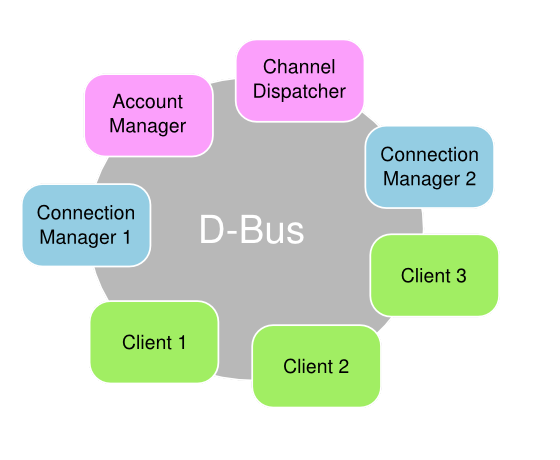
\includegraphics[width=10cm]{fig/telepathy-components-dbus.png}
	\caption{Telepathy components registered with user session D-Bus.\cite{TPWiki}}
	\label{fig:telepathyComponentsDbus}
\end{center}
\end{figure}

The figure \ref{fig:telepathyComponentsDbus}

%\section{Telepathy language bindings}
%Telepathy clients may be written using language bindings. These bindings must provide D-Bus API. 
%Telepathy-glib, Telepathy-python
%Telepathy-qt4

\section{Empathy}
Empathy is a multiprotocol instant messaging application based on Telepathy. In the terms described above Empathy is a Telepathy client. It is written in python using Telepathy-python bindings. Empathy registers a well-known name with D-Bus and communicates with Telepathy components to provide the communication services. Empathy supports text messaging, file transfer, voice and video calls over various protocols. Supported protocol include Google Talk, XMPP/Jabber, MSN, IRC, AIM Facebook, Yahoo!, Gau Gadu, and ICQ. For some of those protocols like Google Talk and XMPP voice and video calls implemented. The suppport of the protocols depend on Telepathy Connection managers installed. Additional functionality includes sharing users' whereabouts among themselves, automatic reconnection when internet connection is reestablished and automatic changes of presence to away and extended away.\cite{empathyGnome}

The current stable version of Empathy is 2.32.2 and it is a default communication application in GNOME releases since version 2.24 instead of Pidgin. Empathy also replaced Ekiga - program for voice calls and video-call. It became an ultimate free communication tool. Empathy's GUI is takes after Gossip, which is an older IM application for GNOME. 

% =========================================================================================================================
% =========================================================================================================================

\chapter{Existing solutions}

%\section{SIP}
%\section{RTP}

There is a number of existing communication applications offering voice calls and shared whiteboard. Some more popular, more advanced, more user-friendly, offering more features or better support than others. Some of those program support video call and some even conference calls. We shall go over the existing solutions that implement both shared whiteboard and voice calls. Among the described are Skype\cite{skype}, Windows Live Messenger\cite{WindowsLiveMessenger}, Brosix\cite{brosix}, Yahoo! Messenger\cite{yahoo} and AIM\cite{AIM}.

\section{Applications with whiteboard and VoIP support}
\subsection*{Skype}
Skype is the most popular and most used common VoIP application of all. Skype was released in 2003 and was developed by KaZaa\cite{kazaa}. It is available for all major computer platforms (Microsoft Widnows, Mac OS X and GNU Linux) as well as mobile platforms like Android and even Apple's iOS. Although skype is available for Linux it is not well supported. The latest version of skype for Linux is 2.1.0.81 Beta while skype for Windows is of version 5.1. Finally skype is built-in on more and more TVs.

Skype communicates using Skype protocol, which is proprietory. Recently much effort is being put in reverse engineering the skype protocol although the first attempt dates back to 2004 and was done in \cite{skypeProtocolAnalysis}. Skype encrypts the communication end-to-end with 256 bit AES so the amount of information acquired by packet sniffers is very limited. The motivation for recent efforts are simple. Skype is used by tens of millions of users every day, but the support for Linux is at this point almost nonexisting. Linux users have had enough and plan to create an open source client capable of communicating with skype. The wikipedia skype protocol page\cite{wikipediaSkypeProtocol} is filling up with details.  

While most of IM programs utilize client-server communication scheme, skype uses peer-to-peer model. The skype network consists of nodes, supernodes and login servers(see figure\ref{fig:skypeArchitecture}). Nodes are clients. Each client keeps addresses of a number of supernodes. Supernodes are clients with good-enough bandwith, public IP address and enough memmory and CPU power. Supernodes forward traffic to clients behind NAT or restrictive filters. It is believed that skype uses something like STUN. STUN helps overcome NAT and was first defined in \cite{STUNRFC} and then superseded by \cite{STUNRFCNEW}. It seems that nodes themselves determine whether they are behind NAT or firewall. If two nodes want to communicate and either of them or both is behind NAT then a supernode is used to forward traffic between them. 

Skype call signalling is done via TCP and UDP is primarily used for the voice transfer. If a skype client finds out it is behind a firewall that forbids UDP, the speech is transferred using TCP. The codec used is unknown although there are couple candidates. What is almost certain is the fact that skype uses wideband codec. 

The decentralized architecture seems to be working well although there was an outage on December 22nd 2010. Skype officials claim it was due to lack of supernodes\cite{skypeOutage}.  


Features of skype include calling landlines and cell phones and sending text messageses and vice versa - SkypeOut and SkypeIn. The feature list continues with voice and video calls, multi-user chat, conference calls, voice mail and screen sharing. The newest and long expected feature of video conference was introduced in may of 2010 in skype 5.0. 

Though closed program, skype provides an API for developers who want to create extensions called skype extras. Skype extras include a wide range of utilities that might be plugged into skype. The extras uSeeToo, TalkAndWrite, WhiteBoardMeeting and Sketch Pad all provide shared whiteboard each in their own way.    

% TCP for signaling and TCP and UDP for transport
% wideband codec 

\begin{figure}[ht]
	\begin{center}
	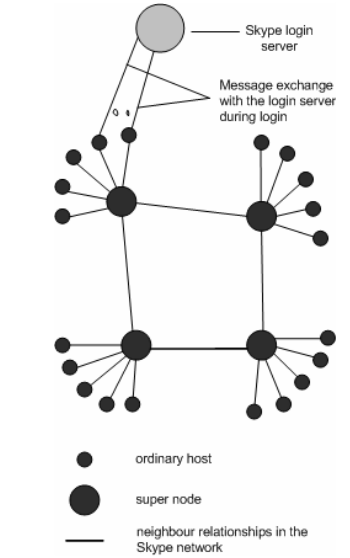
\includegraphics[width=8cm]{fig/skype-architecture.png}
	\caption{Telepathy components registered with user session D-Bus.\cite{skypeProtocolAnalysis}}
	\label{fig:skypeArchitecture}
\end{center}
\end{figure}

\subsection*{Windows Live Messenger}
Windows Live Messenger was first released in July 1999 as MSN Messenger and offered just text messaging with users of AOL Instant Messenger\cite{AIM}. Due to AOL's constant effort to block Microsoft from it's network Microsoft gave in and removed the feature. Since then MSN Messenger could only connect to MSN Messenger Service. In 2001 with the release of Windows XP, MSN Messenger 4.6 came out with voice call support. The last version of MSN Messenger, version 7.5, featured video calls. Windows Live Messenger 8.0 was released in june 2006 and that was the end of the name MSN Messenger.   

Windows Live Messenger utilizes client-server model and communicates using Microsoft Notification protocol over TCP. The first 7 versions of MSNP were disclosed to public, but since version 8 the details have been kept a secret. MSNP does not use encryption so eventhough MSNP's description was not published it was not hard to put it together using packet sniffers.

The live Messenger is available for Windows, Mac OS X and recently was integrated into Microsoft's game console Xbox 360. It features social network integration, offline messaging, games and applications, voice and video calls and standard IM features. An interesting feature is Multiple points of presence allowing user to be connected on two devices. Shared whiteboard is available as an extra application and is not capable of multi-user session.   

\subsection*{Brosix}
An award winning application first released in 2006. Brosix features voice and video chat and multi-user chat, basic IM functions and couple advanced functions. Brosix's whiteboard is an Microsoft Paint like window shared among the participants and won Best IM Feature 2009 award from about.com. Next great feature allows users share screen, including mouse and keyboard much like VNC. Finally Brosix implements co-browsing where users share a browser window. 

Brosix is available for Windows, Max OS X and GNU Linux in commercial and personal(free) version. There is little known about used technologies and it is almost impossbile to reverse-engineer using packet sniffers as Brosix uses 256 bit AES encryption.

\subsection*{Yahoo! Messenger}
Yahoo! Messenger is just like all of the above a closed program though some information has leaked\cite{wikipediaYahoo}. Yahoo! Messenger protocol(YMSG) uses TCP on port 5050 or a different one if default is unavailable. To get to clients behind firewall HTTP is utilized. Video and voice supposedly use SIP and H.323.

Besides the standard set of IM functions Yahoo! Messenger can call PSTN, send SMS and handle voice conference. Whiteboard feature is called Scribbler and is plugin. Linux is missing in the list of supported platforms while Windows and Mac OS X are not.

\subsection*{AOL Instant Messenger}
AIM is yet another IM with proprietory communication protocol. Though AIM is a bit of an exception for it supports two protocols. First is just for simple text messaging called TOC and has been disclosed to public. Second protocol that supports all of the advanced features is being kept a secret.

AOL's messenger is available for Windows and Mac OS X and features voice and video calls as well as whiteboarding. Whiteboard is available as a plugin for AIM called IM Whiteboard. 

\section{Multimedia streaming protocols}
\subsection*{SIP}
Session Initiation Protocol is a standardized by IETF and was firts defined in RFC 2543. The latest definition is in RFC 3261. SIP is used in VoIP for negotiating the details of the call. The parameters of the call are described using Session Description protocol described in RFC 4566. Though designed for VoIP it can be used for establishing or terminating any kind of session whether it is between two users or it is a multiuser session. Among the features of SIP is also instant messaging, presence or any kind of event notification. SIP uses primarily UDP on port 5060, but can also use TCP on the same port and 5061 for TLS secured SIP. The syntax is similar to HTTP.

SIP clients are identified by URI\footnote{Uniform Resource Identifier} which usualy looks like this: \verb|sip:username@hostname|, to be concrete \verb|sip:bob@biloxi.com|. Firts the client must register with a SIP proxy, which in Bob's case is \verb|biloxi.com|. Now let's say Alice wants to call Bob. Todo that she needs to know his URI. She sends an \verb|INVITE| to her SIP proxy, by which it is forwarded to Bob's proxy and finally delivered to Bob and his phone or computer start ringing. If he picks up an appropriate numeric code is sent to Alice. The following example\cite{SIPRFC} shows the scenario presented:    

\lstinputlisting{sip-example.tex}

Since SIP serves only to initiate the session it need to cooperate with a protocol that does transfer the data. That protocol is Real-time Transfer Protocol.  

\subsection*{RTP}
Real-time Transport Protocol is an IETF standard for tranporting data that need to be delivered in real-time rather than reliably. Therefore UDP is used on the transport layer. First was RTP defined in RFC 1889 in 1996 and then later updated in RFC 3550 in 2003. It is primary protocol for streaming audio and video over the internet. It is used for VoIP for transporting the voice while SIP negotioates parameters of the transport. More and more TV stations have been converting to the internet and they use RTP as means of distribution. RTP uses unicast as well as multicast when streaming to multiple subscribers.

RTP is used in conjunction with Real-time Transport Control Protocol. RTCP monitors QoS\footnote{Quality of Service}, statictics of the transfer and help with synchronisation when streaming to multiple destinations. The volume of RTPC traffic should be aroung 5\% of the volume of the stream.  

Unlike the circuit switched network, where the QoS is ensured by it's nature, the packet switched network does not have a way of ensuring short or not even constant delay or sufficient bandwidth. RTP defines mechanisms for making the most of the packet switched network. It is important to note that in packet switched network packet of the same stream might take different path to theis destination. That and network congestion are reason for varying delay commonly reffered to as jitter. RTP labels all the packets with sequence numbers. The implementation of RTP at the destination has a buffer to compensate fo jitter and out of sequence delivery. If the packet arrives too late it is dropped. Dropping packets to some point might not even be noticable by the user. 

RTP sends and receives data on even port numbers and the associated RTCP uses the next higher odd port number. An example on an RTP packet follows. 

\begin{figure}[ht]
	\begin{center}
	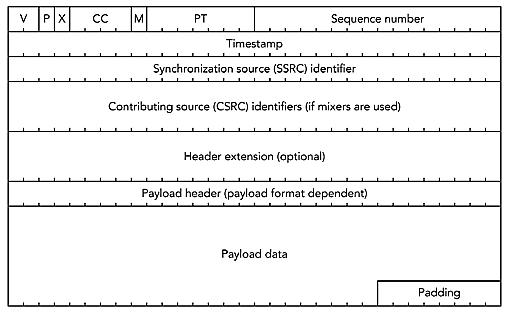
\includegraphics[width=10cm]{fig/rtp-packet.png}
	\caption{RTP packet.\cite{rtpBook}}
	\label{fig:rtpPacket}
\end{center}
\end{figure}

% VoIP
% voice quality factors - codec, echo control, packet loss, delay variation = jitter, QoS
% some codecs may recover from loosing one packet but just one
% delay too long = two separate conversations effect
% jitter buffer to compensate for jitter, if the delays vary too much the buffer overflows and renders the same effect as loosing packets
% voice activity detection and silence suppresion - the codec generates low rate "comfort noise" to make it sound like an actual backround noise from the telephone
% delays caused by coding voice and packetization
% 

% =========================================================================================================================
% =========================================================================================================================

%\chapter{Implementation}

% =========================================================================================================================
% =========================================================================================================================

\chapter{Conclusion}
The world of today can be described as one enormous network, to which everyone is or soon will be connected. One of the Internet's greatest features is bringing people together. People who hundred of years ago would have to travel sometimes months to see each other or wait for reply get an opinion on an idea from a colleague. Today it is just a few clicks away.

Numerous application exist featuring whiteboard and VoIP and some of them even video conferencing. All of the programs mentioned in chapter 5 unfortunately used proprietory protocols and do not provide any information about it at all. 

There are several ways to implement a VoIP solution. RTP with SIP seems to be a feasible solution as it has been proven to work by numerous applications.Though after much thinking it seems the technologie to with will be XMPP Jingle. It has been implemented by Collabora and is now part of Telepathy Gabble - XMPP connection manager. Though still under development the presented result look promising.

There are several tasks to be done. First is porting Makneto to Telepathy. Then a thourough examination of voice encoding must be done to decide what codec shall be used. And finally implementing VoIP support to Makneto.   


 % viz. obsah.tex

  % Pouzita literatura
  % ----------------------------------------------
\ifczech
  \bibliographystyle{czechiso}
\else 
  \bibliographystyle{plain}
%  \bibliographystyle{alpha}
\fi
  \begin{flushleft}
  \bibliography{literatura} % viz. literatura.bib
  \end{flushleft}
  \appendix
  
  \chapter{CD Content}
\textbf{/Makneto/*} - revision of program Makneto from May 23rd 2011\newline
\textbf{/Makneto/README} - manual for compiling Makneto\newline
\textbf{/thesis/*} - source code of this thesis\newline
\textbf{/projekt.pdf} - text of this work\newline
%\chapter{Dependencies}
%\chapter{Konfigrační soubor}
%\chapter{RelaxNG Schéma konfiguračního soboru}
%\chapter{Plakat}

 % viz. prilohy.tex
\end{document}
